\section{Results and Discussion}
\label{sec:Results_and_Discussion}
This section contains lists of all important results and summarizes the most important things.

\begin{table}[H]
	\centering
	\renewcommand{\arraystretch}{1.3}
	\begin{tabular}{r||c|c|c}
		& \textbf{Measured} ($\mu$m) & \textbf{True Value} ($\mu$m) & \textbf{Deviation} (\%) \\
		\hline\hline
		\textbf{Slit 1} & 39.41 $\pm$ 0.93 & 40 & -1.5 \\
		\textbf{Slit 2} & 101.26 $\pm$ 6.77 & 100 & +1.3 \\ \hline
		\textbf{Anti-Slit 1} & 239.10 $\pm$ 23.34 & 230 & +4.0 \\
		\textbf{Anti-Slit 2} & 123.39 $\pm$ 6.80 & 124 & -0.5 \\ \hline
		\textbf{Circular Aperture 1} & 151.39 $\pm$ 10.24 & 150 & +0.9 \\
		\textbf{Circular Aperture 2} & 101.62 $\pm$ 4.60 & 100 & +1.6 \\ \hline
		\textbf{Cross-Grid 1} & 28.53 $\pm$ 0.57 & 28 & +1.9 \\
		\textbf{Cross-Grid 2} & 50.22 $\pm$ 0.30 & 50 & +0.44 \\ \hline
	\end{tabular}
	\caption{Summary of all Results}
	\label{tab:results}
\end{table}

Table \ref{tab:results} shows that all the calculated mean values are really close to their true values (all values are within < 4 \% deviation). The other important thing is to check, wheter their true value lies between the measured value and its uncertainty. This is shown in the following figure \ref{fig:Graphical_Comparison}:

\begin{figure}[H]
	\centering
	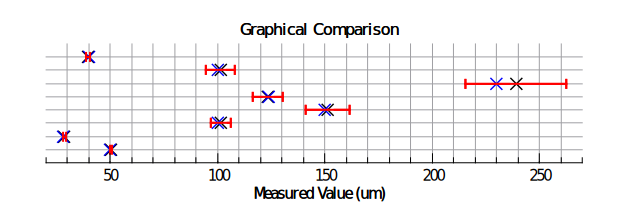
\includegraphics[scale=0.94]{Graphical_Comparison}
	\caption{Graphical Comparison}
	\label{fig:Graphical_Comparison}
\end{figure}

Figure \ref{fig:Graphical_Comparison} shows a graphical comparison between the calculated values (black cross with red uncertainty bar) and their respective true values (blue cross). The display order is the same as in the above table \ref{tab:results}. Although it is difficult to see for the values with a small error bar, \textbf{all their true values lie between their calculated values and their uncertainties}.
